\chapter{Integration}
\label{chp:Integration}


%%%%%%%%%%%%%%%%%%%%%%%%%%%%%%%%%%%%%%%%%
%
% INTRODUCTION
%
%%%%%%%%%%%%%%%%%%%%%%%%%%%%%%%%%%%%%%%%%

In many ways, integration provides the inspiration for hybrid set domains.
As such, many of the techniques we have been using will be very familiar when placed back within their original context.
That being said, notationally, sets and orientation are treated as often treated as distinct objects rather than a single entity.


As a hopefully illustrative example of this, consider a typical definition of the \textbf{definite integral} from an introductory
course in calculus.
Given a function $f$ with real variable $x$ and an interval $[a,b)$ of the (extended) real line
\footnote{ The extended real line denoted $\extendedreal$ is the set of real numbers as well as the points at 
$+\infty$ and $-\infty$} the definite integral
\begin{equation*}
	\int_a^b f(x) \; dx
\end{equation*}
is defined as the signed area bounded by $f$ between $x=a$ and $x=b$.
Generally after a short exposition about Riemann sums, it would then be revealed that if $F$ is an anti-derivative of the
 function $f$ then:
\begin{equation*}
	\int_a^b f(x) \; dx \;=\; F(b)-F(a) \;=\; - (F(a)-F(b)) \;=\; - \int_b^a f(x) \; dx
\end{equation*}


\todo[inline]{vbox}


However this means that previously defining the definite integral using (unoriented) intervals was a bit of a misnomer.
As we saw in the previous chapter, when $a \geq b$, the interval $[a,b) = \{ x \;|\; a \leq x < b \}$ is the empty set.
So the interval itself cannot really be thought of as a part of the definite integral.
If it were the interval itself that we were concerned with then for $a \leq b$, the interval $[b,a)$ is empty.
As are the intervals $[a,a)$, $[\pi, e)$, and$[\infty, -\infty)$.
As these are all different representations of the same interval, and we are considered with the relationship between $f$ and
the interval, then one might argue that, in fact
\begin{equation*}
	\int_b^a f(x) \; dx \;=\; \int_a^a f(x) \; dx \;=\; \int_\pi^e f(x)\;dx \;=\; \int_\infty^{-\infty} f(x) \; dx
\end{equation*}
Obviously this is not the intent but there is a distinct mismatch between the conceptual usefulness of considering
integrals as over an interval.
But when actually using said interval, it is treated as an ordered pair of endpoints disregarding the set itself.


This issue is exasperated working with the more general notation
\begin{equation*}
	\int_X f(x) \; dx
\end{equation*}
which denotes integrating $f$ over a set $X$.
Now there is nothing stopping $X$ from an interval and one would very much like to say that,
\begin{equation*}
	\int_a^b f(x) \; dx \;=\; \int_{[a,b)} f(x) \; dx
\end{equation*}
but there is no analogous translation to $\int_a^b = - \int_b^a$ and so if we made this assertion we would be left with
\begin{equation*}
	\int_{[a,b)} f(x) \; dx 
		= \int_a^b f(x) \; dx 
		= -\int_b^a f(x) \; dx 
		= - \int_{[b,a)} f(x)\; dx 
		= -\int_\emptyset f(x)\;dx 	
		= 0
\end{equation*}
Again, clearly this is not a desired outcome.

\todo[inline]{Instead what is actually intended is an oriented interval}

Another advantage to using oriented sets is a more natural language for manipulating domains of integration than sets.
There is no common understanding of the sum of two sets, but since we have the point-wise sum $\oplus$ for hybrid sets, we simply say that the integral operator is \emph{bi-linear}.
By this we mean, it is linear with respect to both operands: the function it is integrating over:
\begin{equation}
	\int_{X} f(x) + g(x) \; dx = \int_X f(x) \;dx + \int_X g(x) \; dx
\end{equation}
and the domain of integration:
\begin{equation}
	\int_{X\oplus Y} f(x) \; dx = \int_{X} f(x) \; dx + \int_Y f(x) \; dx
\end{equation}
By definition, this immediately gives way to the very useful identities:
\begin{align}
	\int_{[\![a,c)\!)} f(x) \; dx = \int_{[\![a,b)\!)} f(x) \; dx + \int_{[\![b,c)\!)} f(x) \; dx \\
	\int_{[\![a,b)\!)} f(x) \; dx = \int_{\ominus [\![b,a)\!)} f(x) \; dx = - \int_{[\![b,a)\!)} f(x) \; dx
\end{align}
for all $a$, $b$ and $c$.


\todo[inline]{new chapter overview}

In one dimension, many of these changes may seem trivial advances but in higher dimensions, the oriented and measure-theoretic approaches diverge \cite{tao2007differential}.
Using hybrid sets as domains of integration allow us to use the best features of both.
In this chapter we will present an introduce integration over oriented intervals and generalize to oriented $n$-cubes in higher dimensions.
We will also explore the boundary operator and the cubic homology formed by $n$-cubes.
This will provide a base for the following chapter to investigate the cubic singular homology, integration of forms and Stokes' theorem.
In Chapter 6, we will introduce the oriented Lebesgue integral.


\section{Integration over Hybrid Domains}

%%%%%%%%%%%%%%%%%%%%%%%%%%%%%%%%%%%%%%%%%
% RIEMANN
%%%%%%%%%%%%%%%%%%%%%%%%%%%%%%%%%%%%%%%%%

\subsection{Riemann Integral on $k$-rectangles}


\todo[inline]{new intro}
Now that we have oriented $n$-dimensional cubes, we would like to define the integral over one.
For now, we will content ourselves with the Riemann integral and Euclidean volume.
More complex domains and other metrics will be handled in later chapters with push-backs and the Lebesgue integral.
The volume of an oriented $n$-cube in $\mathbb{R}^n$ we define to be the product of its side lengths.
Formally,

\begin{definition}
	Let $[\![\boldsymbol{a}, \boldsymbol{b}]\!]$ be a $k$-cube in $\mathbb{R}^n$ again with $\boldsymbol{a}=(a_1,\ldots, a_n)$ and $\boldsymbol{b}=(b_1,\ldots, b_n)$. 
	We denote the \textbf{volume of $\boldsymbol{[\![a,b]\!]}$} with $\text{vol}$ and define it as:
	\begin{equation}
		\text{vol}(\; [\![\boldsymbol{a}, \boldsymbol{b} ]\!] \;) = (b_1 - a_1) \cdot (b_2 - a_2) \cdot \ldots \cdot (b_n - a_n)
	\end{equation}
\end{definition}

For any $k<n$, a $k$-cube will have volume zero.
In at least one dimension, the cube will be degenerate (i.e. $a_i = b_i$) and so will contribute zero to the product.
Additionally, one can also observe that $\text{vol}( \ominus [\![\boldsymbol{a}, \boldsymbol{b} ]\!]) = - \text{vol}( [\![ \boldsymbol{a}, \boldsymbol{b} ]\!]$.


\begin{figure}[ht]
\caption[Riemann Integral]{Upper and lower Riemann sums shown for the same sequence shown with light and dark rectangles respectively. A function over an oriented interval is Riemann integrable if the two sums converge.}
\centering
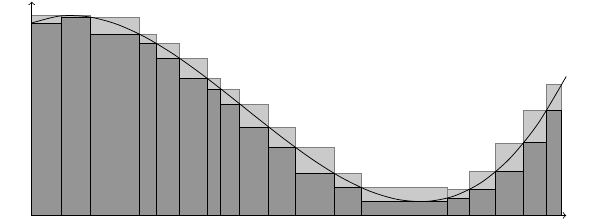
\includegraphics[scale=0.6]{diagrams/riemann}
%\begin{tikzpicture}[scale=2, domain=0:5]
%	\draw[<->] (0,2) -- (0,0) -- (5,0);
%	\draw[smooth,samples=20, domain=0.0:5.0] plot(\x, {(\x^3 - 6 * \x^2 + 4 * \x + 18)/10});
%\end{tikzpicture}
\end{figure}

Given an $n$-cube $[\![\boldsymbol{a}, \boldsymbol{b}]\!]$ we must cut each $[\![a_i, b_i]\!]$ into partitions.
Previously we used generalized partitions and did not mind if pieces overlapped or exceeded the original range.
However, for building our Riemann sums, we are only interested in partitions in the traditional, non-intersecting sense.

\begin{definition}
	Given an oriented interval $[\![a,b]\!]$ of the real line, we say that a partition of $[\![a,b]\!]$, $\{P_i\}_{i=1}^n$
	is an \textbf{interval partition of $\boldsymbol{[\![a,b]\!]}$} if its pieces are:
	\begin{enumerate}
		\item \emph{Oriented intervals}: $P_i$ is an oriented interval of the real line for all $i$.
		\item \emph{Disjoint}: $P_i \otimes P_j = \emptyset$ for all $i,j$
	\end{enumerate}
	We denote the set of all such partition as $\mathcal{P}[\![a,b]\!]$.
\end{definition}

This greatly restricts the types of partitions we have access to.
Every interval partition will be --- up to substitution of ``$]\!], (\!($'' in place of ``$)\!), [\![$'' --- of the form:
\begin{equation}
	\Big\{ \; [\![a,x_1)\!), \; [\![x_1, x_2)\!), \; [\![x_2, x_3)\!),\; \ldots,\; [\![x_{n-1}, b]\!] \; \Big\}
\end{equation}
where $x_i$ is a monotone sequence (that is, either non-increasing or non-decreasing).
This is not to say that $P_i = [\![x_{i-1}, x_i )\!)$ as the pieces of $P$ may not be given in this order.
Regardless of the ordering, we select partitions $P^j \in \mathcal{P}[\![a^j,b^j)\!)$ for each dimension of $[\![a,b)\!)$.
To build our mesh, we construct smaller $n$-cubes $I_{i_1, \ldots, i_n}$ using the Cartesian product of pieces:
\begin{equation}
	I_{i_1, \ldots, i_n} = i_1 \times \ldots \times i_n
\end{equation}
where each $i_j$ is taken from $P^j$.
We are now ready to construct Riemann sums.

\begin{definition}
	Given $P=\{ P_j \}_{j=1}^n$ where $P_j \in \mathcal{P}[\![a_j, b_j]\!]$,
	and $f:[\![\boldsymbol{a}, \boldsymbol{b}]\!] \to \mathcal{R}$ then we define a Riemann sum $f_P$ to be:
	\begin{equation}
		f_P = \sum_{i_1 \in P_1} \ldots \sum_{i_n \in P_n} f(x_{i_1, \ldots, i_n}) \text{vol}(I_{i_1, \ldots, i_n})
	\end{equation}
	where $x_{i_1, \ldots, i_n}$ is any point chosen from $I_{i_1, \ldots, i_n}$.
\end{definition}

Note that we specify \emph{a} Riemann sum, not \emph{the} Riemann sum.
There are several ways to choose $x_{i_1,\ldots,i_n} \in I_{i_1, \ldots, i_n}$ and different samplings can lead to different Riemann sums for the same partition and same function.
In $\mathbb{R}^1$, several common ways to sample include the left and right Riemann sums (which sample at the left and right boundaries), the trapezoidal Riemann sum (which averages the left and right) the upper Riemann sum (which samples at $\max(f(x_{i_1, \ldots, i_n}))$) and the lower Riemann sum (which samples at $\min(f(x_{i_1,\ldots,i_n}))$).

Recall our discussion of refinements from Chapter 2.
Given 2 partitions $P$ and $P'$ of the same set then we say $P \preceq P'$ if $P'$ is a refinement of $P$.
In this way we can induce a partial ordering on $\mathcal{P}[\![a,b]\!]$.
There is a unique smallest element in this partial ordering which is $[\![a,b]\!]$ itself; 
every partition by definition will refine $[\![a,b]\!]$.
Additionally, given $P,P' \in \mathcal{P}[\![a,b]\!]$ then propose that we can always find $Q$ that simultaneously refines both.
If $P=P'$ then trivially $Q=P$ is a common refinement.
Otherwise, we take:
\begin{equation}
	Q= [\![a,b]\!] \otimes \left( \bigoplus_{p\in P} \bigoplus_{p' \in P} p \otimes p' \right)
\end{equation}
The heavy lifting here is done by the fact that every point in $[\![a,b]\!]$ is covered by exactly one $p\in P$ and exactly one $p' \in P$.
The product of any two partition pieces will then be the smallest common interval with multiplicity 1.
Multiplying the entire thing by $[\![a,b]\!]$ is done to correct the sign.
As we go up in our ordering, our mesh becomes increasingly fine.
Taking the Riemann sum of the suprema of this poset gives us the Riemann integral.

\begin{definition}
The Riemann integral of a function $f:\mathbb{R}^n \to \mathbb{R}$ over a $k$-cube $[\![\boldsymbol{a}, \boldsymbol{b}]\!]$
where $P = \sup \Big\{ \mathcal{P} [\![a,b]\!] \Big\}$
	\begin{equation}
		\int_{[\![a,b]\!]} f(x) \; dx = f_P
	\end{equation} 
	We say that a function is \textbf{Riemann integrable} if the upper and lower Riemann sums converge.
\end{definition}

\todo[inline]{redo for arbitrary generalized partition with pieces going to zero}

%%%%%%%%%%%%%%%%%%%%%%%%%%%%%%%%%%%%%%%%%
% DIFFERENTIAL FORMS
%%%%%%%%%%%%%%%%%%%%%%%%%%%%%%%%%%%%%%%%%

\subsection{Differential Forms}

Rather than thinking of integrals as functions over $n$-rectangles, an often more useful language is to use 
\emph{differential forms}.
We define a \textbf{(differential) 0-form} $\beta$ on $\mathbb{R}^n$ as any function 
$\beta : \mathbb{R}^n \to \mathbb{R}$.
And there is very little else to say as they are just functions on $\mathbb{R}^n$.



A \textbf{(differental) 1-form} $\omega$ on $\mathbb{R}^n$ is an expression of the form:
\begin{equation}
	\omega = f_1(\text{x}) \; dx_1 + f_2(\text{x}) \; dx_2 + \ldots + f_n(\text{x}) \; dx_n
\end{equation}
Now this look very much like something we're used to integrating.
Specifically it is something that be used as an integrand over a 1 dimensional domain.
For example, Green's theorem is introduced using differential forms without even mentioning them as such.
\begin{equation}
	\tag{Green's Theorem}
	\textcolor{black!40}{
		\int_D \left( \frac{\partial f_2}{\partial x} - \frac{\partial f_1}{\partial y}  \right) \;dx\;dy 
		=\int_{C}
	} f_1(x,y) \; dx + f_2(x,y) \; dy
\end{equation}
Here $C$ is a closed curve that encloses $D$ a region in the $(x,y)$ plane; hence the right-hand side is an integral of
a 1-form over a 1-dimensional curve.
Having multiple $dx_i$ appearing in a single integrand may initially seem unusual when first presented, 
but is quite intuitively handled.
Integration is linear so just as we can separate $\int f(x) + g(x) dx$ into $\int f(x) dx + \int g(x) dx$, we can similarly break
up an integral of a 1-form into the sum of integrals over \emph{basic} 1-forms (1-forms involving a single term).
\begin{equation}
	\int f_1(\text{x}) \; dx_1 + f_2(\text{x}) \; dx_2 + \ldots + f_n(\text{x}) \; dx_n
	=
	\sum_{i=1}^n \left( \int f_i \; dx_i \right)
\end{equation}


Adding two 1-forms then is quite straight-forward; simply collect terms with matching $dx_i$.
So if we can add differential forms but what about multiplication?
For a 0-form $\beta$ and 1-form $\omega$ as defined above, the answer the answer is a simple yes:
\begin{equation}
	(\beta \cdot \omega)(\text{x}) = \beta(\text{x})f_1(\text{x})dx_1 + \ldots  + \beta(\text{x})f_n(\text{x})dx_n
\end{equation}
The result is a 1-form where each basic 1-form term is the product of $f_i$ and $\beta$ in $\mathbb{R}$.
To ``multiply'' two 1-forms together however we must turn instead to the wedge product $\wedge$.

First of all, the wedge product is primarily defined by being \emph{anti-commutative} or \emph{skew-symmetric}.
That is, $dx \wedge dy = -dy \wedge dx$ and several results will immediately follow.
When applied to two identical $dx$, we have $dx \wedge dx = - dx \wedge dx$ and so $dx \wedge dx = 0$.
Additionally, for any permutation $\sigma$ of $[p]$
\begin{equation}
	dx_1 \wedge ... \wedge dx_p = \text{sgn}(\sigma) \; dx_{\sigma(1)} \wedge ... \wedge dx_{\sigma(p)}
\end{equation}
The wedge product of two 1-forms moves us out of the realm of 1-forms which have basis $dx_i$ and into the 
realm of 2-forms with basis $dx_i \wedge dx_j$.


\begin{definition}
	Given a $k$-rectangle $\Omega \in \mathbb{R}^n$ with coordinates $\text{x} = (x_1, x_2, \ldots, x_n)$
	A \textbf{differential $p$-form} $\beta$ over $\Omega$ has the form:
	\begin{equation}
		\beta = \sum_{j_1 \in [n]} \ldots \sum_{j_p \in [n]} b_{(j_1, \ldots, j_p)}(\text{x}) \; 
				\text{d} x_{j_1} \wedge \ldots \wedge \text{d} x_{j_p}
	\end{equation}
	Typically, we will take $j$ to be the vector $(j_1, \ldots, j_p)$ and express $\beta$ instead as a single sum multi-indexed
	by $j$, $\sum_j b_j(x) \; dx_{j_1} \wedge \ldots \wedge dx_{j_p}$.
	We denote the space of all $p$-forms on $\Omega$ by $\Lambda^p(\Omega)$.
\end{definition}


\begin{definition}
	Let $\alpha = \sum_i a_i(x) \; dx_{i_1} \wedge \ldots \wedge dx_{i_p} \in \Lambda^p(\Omega)$ and 
	$\beta = \sum_j b_j(x) \; dx_{j_1} \wedge \ldots \wedge dx_{j_q} \in \Lambda^q(\Omega)$. We extend the
	wedge product $\wedge : \Lambda^p(\Omega) \times \Lambda^q(\Omega) \to \Lambda^{p+q}(\Omega)$ by:
	\begin{equation}
		\alpha \wedge \beta  = \sum_{i,j} a_i(x) b_j(x) \; 
			dx_{i_1} \wedge \ldots \wedge dx_{i_p} \wedge 
			dx_{j_1} \wedge \ldots \wedge dx_{j_q}
	\end{equation}
\end{definition}

Although we take all possible $\binom{n}{q} \cdot \binom{n}{p}$ pairs of 
$a_i (x) dx_{i_1} \wedge \ldots \wedge dx_{i_p}$ and $b_i (x) dx_{i_1} \wedge \ldots \wedge dx_{i_p}$,
most of the possible terms will end up being zero.
If \emph{any} of the terms in $dx_{i}$ appears in $dx_{j}$, then the wedge product will be zero 
and no term will be contributed.
As such, if $q+p > n$, there will be a duplicate in every term and so the entire sum will be zero.
When all is said and done, at most we will have $\binom{n}{p+q}$ terms.
Rather than the skew-symmetry we had when commuting $dx \wedge dy$, in higher dimensions the sign depends on 
$p \cdot q$ of the $p$-form and $q$-form we are commuting.
Specifically, 
\begin{equation}
	\alpha \wedge \beta = (-1)^{pq} \beta \wedge \alpha
\end{equation}
This can be easily seen by commuting each of $dx_{j_1}, \ldots dx_{j_q}$ terms each past 
$dx_{i_1}\wedge \ldots \wedge dx_{i_p}$. 
So we are commuting $q$ terms each past $p$ terms, reversing the sign each time for a net $(-1)^{pq}$.


The wedge product is only one part of our algebra of differential forms.
We have several other nice identities for its behaviour with addition and multiplication.
For the following, we consider $f$ to be a function on $\mathbb{R}^n$.
Additionally we consider the differential forms $\omega_1$ and $\omega_2$ to be $k$-forms, $\alpha$ to be a $p$-form
 and $\beta$ to be an $q$-form.
Then we have the following:
\begin{align}
	(\omega_1 + \omega_2) \wedge \alpha  & \;=\; \omega_1 \wedge \alpha + \omega_2 \wedge \alpha \\
	(\omega_1 \wedge \alpha) \wedge \beta & \;=\; \omega_1 \wedge ( \alpha \wedge \beta ) \\
	(f \cdot \omega_1) \wedge \alpha & \;=\;  f \cdot (\omega_1 \wedge \alpha) \;=\; \omega_1 \wedge (f \cdot \alpha)
\end{align}
These should all be quite obvious from definitions. 
We should also note the identities which are \emph{not} present.
We have defined the sum of $\omega_1$ and $\omega_2$: two differential forms which are the same dimension but not
the sum of $\alpha$ and $\beta$: differential forms with different dimension.
It is clear how one would add two differential forms of the same dimension as both were defined as sums to begin with.
We also do not define the multiplication of $\cdot$ two differential forms but we multiplying a form by a function is simply:
\begin{equation}
	(f \cdot \alpha) (x) = \sum_i f(x)\cdot a_i(x) \; dx_{i_1} \wedge \ldots \wedge dx_{i_p}
\end{equation}


Integrating over a $k$-form is quite simple.
First we shall consider integrating a $k$-form over a $k$-rectangle in $\mathbb{R}^k$.
Such a $k$-form is also known as a \emph{top-dimensional form}.
As we saw previously, any form of higher degree must be zero.
If $\omega$ is such a top form then we can always write
\begin{equation}
	\omega = f \; dx_1 \wedge \ldots \wedge dx_k
\end{equation}
for some function $f$.
Other presentations of $\omega$ exist, but we can always achieve such a presentation by commuting over $\wedge$ 
to the canonical ordering $x_1, \ldots, x_n$.
Once we have the $k$-form in this presentation, we just remove the wedges and evaluate the integral using the
integrand $f \; dx_1 \;dx_2 \ldots dx_k$.

\begin{definition}
Let $\alpha$ be a $k$-form on $\Omega \subset \mathbb{R}^n$ of the form $\alpha = A(x) \; \text{d}x_1 \wedge ... \wedge \text{d} x_n$.
If $A \in \mathcal{L}^1 (\Omega , \text{d}x)$ then we define:
\begin{equation}
\int_\Omega \alpha = \int_\Omega A(x) \; \text{d}x
\end{equation}
Where the left-hand side is the integral of a $k$-form and the right-hand side is a Lebesgue integral.
For any $\beta \in \Lambda^k (\Omega)$ we extend this definition linearly as the sum of integrals.
\end{definition}

\begin{definition}
Exterior derivative
\end{definition}

\todo[inline]{...}

\begin{equation}
d(\alpha \wedge \beta) = (d \alpha) \wedge \beta + (-1)^j \alpha \wedge ( d \beta)
\end{equation}


%%%%%%%%%%%%%%%%%%%%%%%%%%%%%%%%%%%%%%%%%
% SINGULAR CUBE
%%%%%%%%%%%%%%%%%%%%%%%%%%%%%%%%%%%%%%%%%
\subsection{Singular Cubes}

Up until now we have been dealing with the very small set of axis aligned $k$-rectangles 
which is a very limiting class to be restricted to.
Instead we would like to be able to integrate over $k$-rectangles that are deformed by some smooth function.
So assume that we have $X \subset \mathbb{R}^m$ and $Y \subset \mathbb{R}^n$ and a smooth map 
 $\varPhi : X \to Y$.
Not only can we map points from $X$ to points in $Y$ but we can \emph{push foward} vectors from $X$ to vectors in $Y$
and with them, push forward tangent spaces as well.


\begin{definition}
	We denote the \textbf{standard $\boldsymbol{k}$-cube} as the specific $k$-rectangle $[\![0,1]\!]^k$ in 	
	$\mathbb{R}^n$ which is the Cartesian product of $k$ copies of $[\![0,1]\!]$.
	We also consider $[\![0,1]\!]^0 = \{0\}$.
	Given an $n$-dimensional manifold $M$, a \textbf{singular $\boldsymbol{k}$-cube in $\boldsymbol{M}$} is a 
	smooth differentiable map $c$ from the standard $k$-cube to $M$, $c:[\![0,1]\!]^k$
	\todo[inline]{Singular $k$-cube: differentiable map $c$ from standard $k$-cube to $k$-dimensional manifold.}
\end{definition}


It is a common abuse of notation to use $c$ to also to refer to the image $c( [\![ 0,1]\!]^k ) \subseteq M$.
The choice of using specifically the standard $k$-cube is arbitrary.
A differentiable map $f$ from $[\![a,b]\!]$ can always be composed with $g:t \mapsto ta +(1-t)b$ 
to get singular cube $c=f \circ g$.
Gives us innumerably more shapes to work with.
Hemisphere for example is the singular 2-cube given by $(r, \varphi) \to r \cos(\pi \varphi) x+ r \sin(\pi \varphi) y$


However if we have a valid integral $\int_{\Omega} \omega$ with $\Omega$ in some space $X$, 
if we push forward $\Omega$ by some function $c$ to another space $Y$, 
then the integral $\int_{c(\Omega)} \omega$ is no longer valid.
The differential form $\omega$ was expressed in coordinates for $X$ but now that the domain of the integral is in $Y$,
we must perform a change of coordinates.
The true reason why we use differential forms is how cleanly they handle this change in coordinates 
through the use of pull-backs.

Informally, a pullback is a \emph{reversed} function composition.
In typical function composition $(f \circ g)(x) = f(g(x))$, for input $x$ one first evaluates the second function $g$ at $x$
before feeding the result of $g(x)$ into the first function $f$.
The pre-composition or pullback would be $f^*g = g(f(x))$. 
One first evaluates the first function and feeds the result into the second.
Gets its name from pulling $f$ back through $g$.


\todo[inline]{pullbacks and forms}

\begin{equation}
F^* (\alpha \wedge \beta ) = (F^* \alpha) \wedge (F^* \beta)
\end{equation}

\begin{equation}
F^* (d \beta ) = dF^* \beta
\end{equation}

\todo[inline]{vbox}


If we again have $\beta = \sum_j b_j(\text{x}) dx_{j_1} \wedge \ldots \wedge dx_{j_k} \in \Lambda^k(\Omega)$
and some \todo{smooth + differentiable?} map $F: X \to \Omega$.
The pull-back of $\beta$ is
\begin{equation}
F^* \beta = \sum_j  b_j ( F(x)) (F^* \text{d}x_{j_1}) \wedge ... \wedge (F^* \text{d} x_{j_k})
\end{equation}
and
\begin{equation}
F^* \text{d}x_j = \sum_\ell \frac{\partial F^j}{\partial x_\ell} \; \text{d} x_\ell
\end{equation}

Which can be reduced by:
\begin{align}
F^ * \beta & = \sum_j  b_j ( F(x)) (F^* \text{d}x_{j_1}) \wedge ... \wedge (F^* \text{d} x_{j_k}) \\
& = \sum_j  b_j ( F(x))  
\left( \sum_\ell \frac{\partial F^{j_1}}{\partial x_\ell} \; \text{d} x_\ell \right)
\wedge ... \wedge  
\left( \sum_\ell \frac{\partial F^{j_k}}{\partial x_\ell} \; \text{d} x_\ell \right) \\
& = \sum_j b_j ( F(x)) \; \text{det}\left( J_F \right) \; \text{d}x_{j_1} \wedge ... \wedge \text{d} x_{j_k}
\end{align}

Which is significant given the change of variable formula for integration:

\begin{equation}
\int_{\phi(U)} \! f(v) \; dv = \int_U \! f(\phi(u)) \; |\text{det}\phi'(u)| \; du
\end{equation}

\begin{theorem}
Let $F : X  \to \Omega$ be an (orientation-preserving diffeomorphism) and $\alpha$ an integrable $n$-form on $\Omega$ then
\begin{equation}
\int_{F(X)} \alpha = \int_X F^* \alpha
\end{equation}
\end{theorem}




To integrate over a manifold $M$, we first observe that each local chart in the manifold is essentially a singular cube.
If the chart is not a map over the standard cube, then there exists a diffeomorphism 
that can be composed with the local map to transform it into a singular cube.
It is then a matter of stitching together these local charts so that points in the manifold are not ``double-counted''.
To do this we use a partition of unity on $M$: a collection of functions $\theta_k \geq 0$ such that 
for all points in $x \in M$, $\sum_k \theta_k(x) = 1$.
In addition we also enforce that for each function $\text{supp} \theta_k$ and that at each point in $M$, there are only
a finite number of functions such that $\theta_k \neq 0$.

$\{ \psi_i \}$ a partition of unity with locally finite cover $\{ U_i, \psi_i \}$ of consistently oriented coordinate charts.

\begin{equation}
\int_M \alpha = \sum_i \int_{U_i} \psi_i \alpha
\end{equation}


%%%%%%%%%%%%%%%%%%%%%%%%%%%%%%%%%%%%%%%%%
%
% STOKES' THEOREM
%
%%%%%%%%%%%%%%%%%%%%%%%%%%%%%%%%%%%%%%%%%
\section{Stokes' Theorem}

When discussing differential forms an equation called \emph{Green's Theorem} was shown. 
Green's Theorem allows for one to convert between an integral over a 2-dimensional region and a 1-dimensional integral
over a curve that bounds it.
This turns out to be just one instance of the more general \emph{Stokes' Theorem} 
which will work in higher dimensions as well.
To do so we will first need to generalize the notion of a bounding region or boundary.



%%%%%%%%%%%%%%%%%%%%%%%%%%%%%%%%%%%%%%%%%
% BOUNDARY
%%%%%%%%%%%%%%%%%%%%%%%%%%%%%%%%%%%%%%%%%
\subsection{Boundary Operator}


In one dimension, the boundary of an interval was quite straight-forward.
For a positively oriented interval, the boundary was composed of two points; 
the right end-point was positive and the left end-point was negative.
From the perspective of $k$-rectangles, 
the $\partial$ operator has mapped an oriented 1-rectangle to a set of oriented 0-rectangles.
We will now generalize the boundary to map an oriented $n$-rectangle to an $(n-1)$-rectangle.


\begin{definition}
	Let  $[\![\boldsymbol{a}, \boldsymbol{b}]\!]$ be a a $k$-rectangle in $\mathbb{R}^n$.
	Additionally, let $i_1, i_2, \ldots, i_k$ be the unique non-decreasing sequence of indices such that $a_{i_j} \neq b_{i_j}$.
	The \textbf{boundary of $ \boldsymbol{[\![ a,b ]\!]} $ }, denoted the operator $\partial$ is given by
	\begin{align}
		\partial \left( [\![ \boldsymbol{a}, \boldsymbol{b} ]\!] \right) 
		= \bigoplus_{j=1}^k (-1)^j \;
			\left(	
				[\![ 	(\boldsymbol{a}^{[\![1,n]\!]}), 
					\;\;\;
					(\boldsymbol{b}^{[\![1,i_j)\!)} 
						\oplus \boldsymbol{a}^{\hset{i_j}}
						\oplus \boldsymbol{b}^{(\!(i_j,n]\!]}) 
				]\!] \right.\;
			\notag\\
			\ominus \left.
				[\![ 	(\boldsymbol{a}^{[\![1,i_j)\!)}
						\oplus \boldsymbol{b}^{\hset{i_j}}
						\oplus \boldsymbol{a}^{(\!(i_j, n]\!]}), 
					\;\;\;		 
					(\boldsymbol{b}^{[\![1,i_j)\!)}) 			
				]\!]
			\right)
	\end{align}
\end{definition}


The above equation will require a bit of unpacking to digest featuring oriented intervals in two different contexts.
The first appears in the superscripts of $\boldsymbol{a}$ and $\boldsymbol{b}$. 
The intervals $[\![1, i_j)\!)$ and $(\!(i_j, n]\!]$ are  and is an interval over vector indices just as in Chapter 3.
Thus, the term $\boldsymbol{a}^{[\![1,i_j)\!)}$ refers to the vector $(a_1, a_2, \ldots, a_{i_j-1})$ 
while the term $\boldsymbol{b}^{(\!(i_j,n]\!]}$ refers to $(b_{i_j+1}, b_{i_j+2}, \ldots, b_{n})$.
This provides a compact notation to partition the original range of indices into 3 pieces: $[\![ 1,i_j )\!)$, $\hset{i_j}$, and $(\!(i_j, n]\!]$.
Formally, we are actually using the hybrid sets $\hset{(i_j)^1}$ but we omit multiplicity of one (and will continue to do so through out the section) to lighten notation.


Next we use the pointwise sum $\oplus$ we reconstruct $n$-dimensional vectors from our pieces.
We then construct a $(k-1)$-rectangle using these vectors as in (4.8).
Hence we will have terms of the forms:
\begin{align}
	[\![a_1, b_1]\!]
	\times \ldots \times
	[\![a_{i_{j-1}}, b_{i_{j-1}}]\!]
	\times
	[\![a_{i_j}, a_{i_j}]\!]
	\times
	[\![a_{i_{j-1}}, b_{i_{j-1}}]\!]
	\times \ldots \times
	[\![a_n, b_n]\!]
	\\
	[\![a_1, b_1]\!]
	\times \ldots \times
	[\![a_{i_{j-1}}, b_{i_{j-1}}]\!]
	\times
	[\![b_{i_j}, b_{i_j}]\!]
	\times
	[\![a_{i_{j-1}}, b_{i_{j-1}}]\!]
	\times \ldots \times
	[\![a_n, b_n]\!]
\end{align}


In each Cartesian product, the terms at $i_j$: $[\![a_{i_j}, a_{i_j}]\!]$ and $[\![b_{i_j}, b_{i_j}]\!]$ are both 0-cubes.
Since we defined the sequence $i_j$ by $a_{i_j} \neq b_{i_j}$, 
these 0-rectangles are replacing 1-cubes in $[\![\boldsymbol{a}, \boldsymbol{b}]\!]$.
Hence we are indeed left with a $(k-1)$-cube.




%%%%%%%%%%%%%%%%%%%%%%%%%%%%%%%%%%%%%%%%%
% BOUNDARY OF A 1-RECTANGLE
%%%%%%%%%%%%%%%%%%%%%%%%%%%%%%%%%%%%%%%%%
\subsection{Example: \emph{Boundary of a 1-rectangle}}
Let $\boldsymbol{a}= (a_1)$ and $\boldsymbol{b} = (b_1)$ be trivial 1-tuples. 
Then $[\![\boldsymbol{a}, \boldsymbol{b}]\!] = [\![a_1, b_1]\!]$
It follows that:
\begin{align*}
	\partial ( \; [\![ \boldsymbol{a}, \boldsymbol{b} ]\!] \; )
	=& \; (-1)^i ( [\![\boldsymbol{a}^{[\![1,1)\!)}, \boldsymbol{b}^{[\![1,1)\!)} ]\!]
	\times \hset{a_1} \times
	[\![\boldsymbol{a}^{(\!(1,1]\!]}, \boldsymbol{b}^{(\!(1,1]\!]} ]\!]\\
	&\; \ominus
	[\![\boldsymbol{a}^{[\![1,1)\!)}, \boldsymbol{b}^{[\![1,1)\!)} ]\!]
	\times \hset{b_1} \times
	[\![\boldsymbol{a}^{(\!(1,1]\!]}, \boldsymbol{b}^{(\!(1,1]\!]} ]\!] )\\
	=& \; \ominus [\![\boldsymbol{a}^{\emptyset}, \boldsymbol{b}^{\emptyset} ]\!]
	\times \hset{a_1} \times
	[\![\boldsymbol{a}^{\emptyset}, \boldsymbol{b}^{\emptyset} ]\!]\\
	& \; \oplus
	[\![\boldsymbol{a}^{\emptyset}, \boldsymbol{b}^{\emptyset} ]\!]
	\times \hset{b_1} \times
	[\![\boldsymbol{a}^{\emptyset}, \boldsymbol{b}^{\emptyset} ]\!] \\
	=& \; \hset{b_1} \ominus \hset{a_1} \\
	=& \; \hset{a^{-1}, b^{1}}
\end{align*}

One may notice a relationship between this result and the fundamental theorem of calculus:
\begin{equation}
	\int_a^b F'(x) \; dx = F(b) - F(a)
\end{equation}
Which one could easily rewrite as $\int_{[\![a,b]\!]} F'(x) \; dx = \sum (\partial([\![a,b]\!]))$.
Indeed, this is why we have defined the boundary function as such, but more general statements await.
We defined the boundary for not just intervals on $\mathbb{R}$ but $k$-cubes in $\mathbb{R}^n$.




%%%%%%%%%%%%%%%%%%%%%%%%%%%%%%%%%%%%%%%%%
% BOUNDARY OF A 3-RECTANGLE
%%%%%%%%%%%%%%%%%%%%%%%%%%%%%%%%%%%%%%%%%
\subsection{Example: \emph{Boundary of a 3-rectangle}}
Let $\boldsymbol{a} = (0,0,0)$ and $\boldsymbol{b} = (1,1,1)$.
Omitting the intermediate step, we find the boundary of $[\![ \boldsymbol{a}, \boldsymbol{b} ]\!]$ to be:
\begin{align*}
	\partial ( \; [\![ \boldsymbol{a} , \boldsymbol{b} ]\!] \; ) =
	& 	\; \ominus \; \left( \hset{0} \times [\![0,1]\!] \times [\![0,1]\!] \right)
		\; \oplus \; \left( \hset{1} \times [\![0,1]\!] \times [\![0,1]\!] \right)
	\\& 	\; \oplus \; \left( [\![0,1]\!] \times \hset{0} \times [\![0,1]\!] \right)
	 	\; \ominus \; \left( [\![0,1]\!] \times \hset{1} \times [\![0,1]\!] \right)
	\\& 	\; \ominus \; \left( [\![0,1]\!] \times [\![0,1]\!] \times \hset{0} \right)
	  	\; \oplus \; \left( [\![0,1]\!] \times [\![0,1]\!] \times \hset{1} \right)
\end{align*}

This may not be the most enlightening expression on its own.
In Figure 4.3 below, the 3-rectangle given by $[\![\boldsymbol{a}, \boldsymbol{b}]\!]$ can be seen as a cube in three dimensions.
Physically, the 3-rectangle is a solid cube and includes all interior points.
The boundary meanwhile are just the rectangular outer faces, which conveniently,
 there are also six to match the six terms of $\partial[\![\boldsymbol{a},\boldsymbol{b}]\!]$.

\begin{figure}[ht]
\caption[Unit cube with boundary]{The unit cube in $\mathbb{R}^3$ with positive orientation can be represented as the 3-rectangle: $[\![(0,0,0), (1,1,1) ]\!]$ is shown as a wire-frame. 
The six faces that make up its boundary are shaded and labeled with their corresponding terms.
%Now with 100% more right-handed
}
\centering
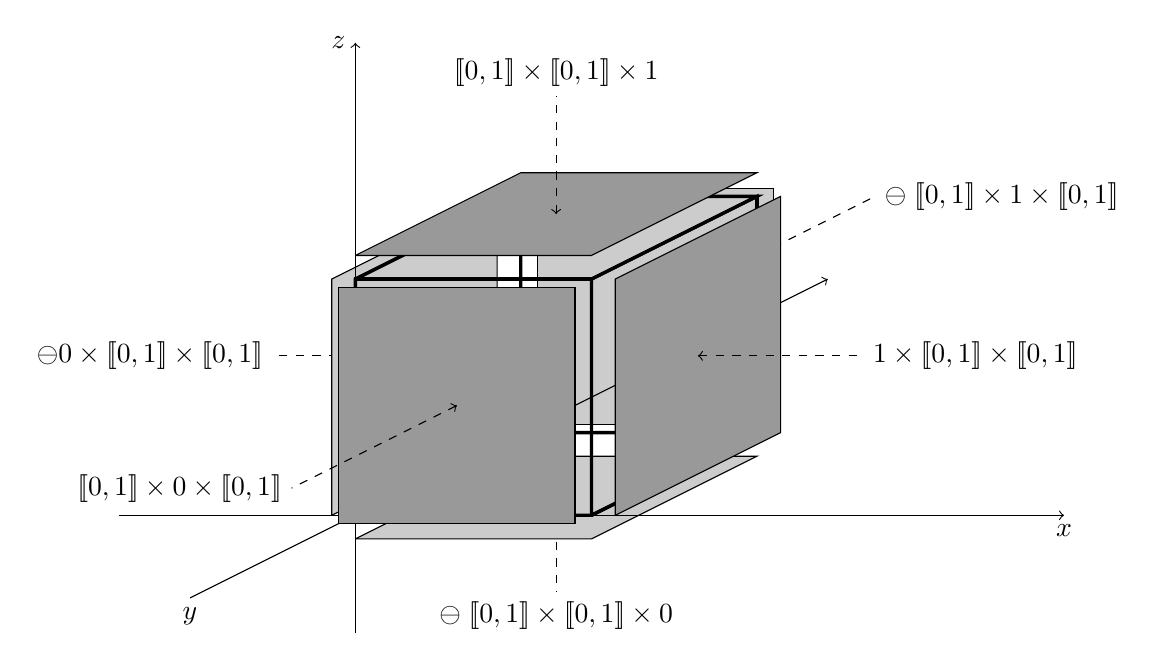
\begin{tikzpicture}[y=1.5cm, x=3cm]	
 	%axis
 	
 	%left
	\draw[color=black, dashed, <-] (0.35, 1.35) --++ (-0.7, 0) node[anchor=east, black] {$\ominus \hset{0} \times [\![0,1]\!] \times [\![0,1]\!]$};
	%back
	\draw[color=black, dashed, <-] (1.2,1.7) --++ (1,1) node[anchor=west, black] {$\ominus \; [\![0,1]\!] \times \hset{1} \times [\![0,1]\!]$};
	%bottom
	\draw[color=black, dashed, <-] (0.85,0.35) --++ (0,-1) node[anchor=north, black] {$\ominus \; [\![0,1]\!] \times [\![0,1]\!] \times \hset{0}$};
 	
 	\filldraw[fill=black!20] (0,-0.2) --++ (1,0) --++ (0.7,0.7) --++ (-1,0) --++ (-0.7,-0.7);
	\filldraw[fill=black!20] (0.77,0.77) --++ (1,0) --++ (0,2) --++ (-1,0) --++ (0, -2);
	\filldraw[fill=black!20] (-0.1,0) --++ (0,2) --++ (0.7,0.7) --++ (0,-2) --++ (-0.7,-0.7);
 	
	\draw[->] (-1,0) -- coordinate (x axis mid) (3,0) node[anchor=north] {$x$};
    	\draw[->] (0,-1) -- coordinate (y axis mid) (0,4) node[anchor=east] {$z$};
	\draw[->] (-0.7,-0.7) node[anchor=north] {$y$} --++ (2.7,2.7) ;
	
	\draw[very thick] (0,0) --++ (1,0) --++ (0.7,0.7) --++ (-1,0) --++ (-0.7,-0.7);
	\draw[very thick] (0.7,0.7) --++ (1,0) --++ (0,2) --++ (-1,0) --++ (0, -2);
	\draw[very thick] (0,0) --++ (0,2) --++ (0.7,0.7) --++ (0,-2) --++ (-0.7,-0.7);
	\draw[very thick] (0,2) --++ (1,0) --++ (0.7,0.7) --++ (-1,0) --++ (-0.7,-0.7);
	\draw[very thick] (0,0) --++ (1,0) --++ (0,2) --++ (-1,0) --++ (0, -2);
	\draw[very thick] (1,0) --++ (0,2) --++ (0.7,0.7) --++ (0,-2) --++ (-0.7,-0.7);
	
	\filldraw[fill=black!40] (0,2.2) --++ (1,0) --++ (0.7,0.7) --++ (-1,0) --++ (-0.7,-0.7);
	\filldraw[fill=black!40] (-0.07,-0.07) --++ (1,0) --++ (0,2) --++ (-1,0) --++ (0, -2);
	\filldraw[fill=black!40] (1.1,0) --++ (0,2) --++ (0.7,0.7) --++ (0,-2) --++ (-0.7,-0.7);

	%right
	\draw[color=black, dashed, <-] (1.35+0.1, 1.35) --++ (0.7, 0) node[anchor=west, black] {$\hset{1} \times [\![0,1]\!] \times [\![0,1]\!]$};
	%front
	\draw[color=black, dashed, <-] (0.5-0.07,1-0.07) --++ (-0.7,-0.7) node[anchor=east, black] {$[\![0,1]\!] \times \hset{0} \times [\![0,1]\!]$};
	%top
	\draw[color=black, dashed, <-] (0.85,2.35+0.2) --++ (0,1) node[anchor=south, black] {$[\![0,1]\!] \times [\![0,1]\!] \times \hset{1}$};
\end{tikzpicture}
\end{figure}

There are several ways to interpret and visualize the $\oplus$ and $\ominus$ sign associated with each face.
Most naturally in $\mathbb{R}^3$ for 2-rectangles is to give each a front and back side with the sign determining which to use.
Alternatively, a 2-rectangle has a boundary formed by 1-rectangles which when drawn as arrows, will all meet head-to-tail.
This induces a clockwise or counter-clockwise cycle around the edge of the rectangle and so $\circlearrowright$ and $\circlearrowleft$ are also commonly used.
This can be seen in Figure 4.4.
One may even notice that the normals produced by both are the same and choose to use that.
These are all conceptual tools, which are convenient to use particularly in $\mathbb{R}^2$ and $\mathbb{R}^3$.
There may not be such a nice physical interpretation in other spaces.


\begin{figure}[ht]
\caption[Orientations of 2-rectangles]{One way of visualizing the orientation of 2-rectangles using clockwise and counter-clockwise cycles of arrows for 1-rectangles. 
The boundary of $[\![a,b]\!] \times [\![c,d]\!]$ becomes the cycle: 
$(a,c) \to (b,c) \to (b,d) \to (a,d) \to (a,c)$.
Showing the relationship between $[\![a,b]\!] \times [\![c,d]\!]$ and $[\![b,a]\!] \times [\![d,c]\!]$ }
\centering
\begin{tikzpicture}

	\def\rectCycle#1#2#3#4{
		\draw[thick, ->, color=black!80] (#1,#2) -- (#3,#2);
		\draw[thick, ->, color=black!60] (#3,#2) -- (#3,#4);
		\draw[thick, ->, color=black!40] (#3, #4) -- (#1,#4);
		\draw[thick, ->, color=black!20] (#1,#4) -- (#1,#2);
		\draw[thick, ->] (#1, 0) -- (#3, 0);
		%\draw[fill] (#1,#2) circle (1 pt);
	}

	
	\rectCycle {0+1}{1} {0+2}{2};
	\draw[<->] (0,3) -- (0,0) -- (3,0);
	\draw[very thick, ->] (0,1) -- (0,2);
	\draw (0,1.5) node[anchor=east] {$+$};
	\draw (1.5,0) node[anchor=north] {$+$};
	%\draw (1.5, 1.5) node {$+$};
	\draw(1.5,1.5) node {$\;\circlearrowleft^+$};
	
	  
	\rectCycle {4+2}{1} {4+1}{2};
	\draw[<->] (4+0,3) -- (4+0,0) -- (4+3,0);
	\draw[very thick, ->] (4+0,1) -- (4+0,2);
	\draw (4+0,1.5) node[anchor=east] {$+$};
	\draw (4+1.5,0) node[anchor=north] {$-$};
	%\draw (4+1.5, 1.5) node {$-$};
	\draw(4+1.5,1.5) node {$\;\circlearrowright^-$};
	
	
	\rectCycle {8+2}{2} {8+1}{1};
	\draw[<->] (8+0,3) -- (8+0,0) -- (8+3,0);
	\draw[very thick, ->] (8+0,2) -- (8+0,1);
	\draw (8+0,1.5) node[anchor=east] {$-$};
	\draw (8+1.5,0) node[anchor=north] {$-$};
	%\draw (8+1.5, 1.5) node {$+$};
	\draw(8+1.5,1.5) node {$\;\circlearrowleft^+$};
	
	
	\rectCycle {12+1}{2} {12+2}{1};
	\draw[<->] (12+0,3) -- (12+0,0) -- (12+3,0);
	\draw[very thick, ->] (12+0,2) -- (12+0,1);
	\draw (12+0,1.5) node[anchor=east] {$-$};
	\draw (12+1.5,0) node[anchor=north] {$+$};
	%\draw (12+1.5, 1.5) node {$-$};
	\draw(12+1.5,1.5) node {$\;\circlearrowright^-$};
	
\end{tikzpicture}
\end{figure}


%%%%%%%%%%%%%%%%%%%%%%%%%%%%%%%%%%%%%%%%%
%
% CHAINS
%
%%%%%%%%%%%%%%%%%%%%%%%%%%%%%%%%%%%%%%%%%
\subsection{Chains}

In fact, we have already seen $k$-chains without mentioning them explicitly.
The boundary of a $k$-cube was the sum $\oplus$, of $2k$ $(k-1)$ cubes.
Chains do not have to be boundaries however, any linear combination of $k$-cubes will do.


\begin{definition}
We denote the Abelian group of of all $k$-cubes in $X$ as $C_k(X)$ (omitting $X$ when obvious by context).
An element $c \in C_k$(X) is called a \textbf{$\boldsymbol{k}$-chain on $X$} and is of the form:
\begin{equation}
	c = \bigoplus_{c_i \in X} \lambda_i c_i
\end{equation}
with integer coefficients $\lambda_i$ and  $k$-cubes in $c_i$.
If coefficients $\lambda_i$ are $\pm 1$ and $c$ is \emph{locally finite} (i.e. each $c_i$ intersects with only finitely many $c_j$ that have non-zero coefficients) then we say that $c$ is a \textbf{domain of integration}.
\end{definition}
	
	
Since $k$-chains are just linear combinations of $k$-cubes, we naturally extend many of our definitions linearly as well.
The integral $\int_c f$ of a $k$-chain $c=\bigoplus_i \lambda_i c_i$ is defined as $\lambda_i \int_{c_i} f  + \lambda_2 \int_{c_2} f + \ldots$.
Doing the same for the boundary operator $\partial$ we have:
\begin{align*}
	&\partial_k: C_k \to C_{k-1} \\
	&\partial_k(c) = \bigoplus_{i=1}^k \lambda_i \partial_k(c_i)
\end{align*}
Elegantly, the boundary operator now maps $k$-chains to $(k-1)$-chains!
\begin{equation}
	\ldots \xleftarrow{\partial_{k-1}} C_{k-1} \xleftarrow{\partial_{k}} C_k \xleftarrow{\partial_{k+1}} C_{k+1} \xleftarrow{\partial_{k+2}} ...
\end{equation}
The most natural next question becomes \emph{``What does $\partial_{k-1}( \partial_k ( c ))$ look like?''}




%%%%%%%%%%%%%%%%%%%%%%%%%%%%%%%%%%%%%%%%%
% BOUNDARY OF A BOUNDARY
%%%%%%%%%%%%%%%%%%%%%%%%%%%%%%%%%%%%%%%%%
\subsection{Example: \emph{Boundary of a boundary (of a 2-cube)}}
Let $\boldsymbol{a} =(a_1,a_2)$ and $\boldsymbol{b}= (b_1,b_2)$.
We wish to compute $\partial_1 ( \partial_2 ( \; [\![\boldsymbol{a}, \boldsymbol{b} ]\!] \; ) )$
\begin{align}
	\partial_1 ( \partial_2 ( [\![ a_1 , b_1 ]\!] \times [\![a_2, b_2 ]\!] ) )
	=	& 	\; \ominus 	\partial_1( \hset{0} \times [\![0,1]\!]) 
			\; \oplus \; 	\partial_1(\hset{1} \times [\![0,1]\!]) \notag \\
		& 	\; \oplus 	\partial_1( [\![0,1]\!] \times \hset{0}) 
			\; \ominus \; \partial_1([\![0,1]\!] \times \hset{1}) \\
	=	& 	\ominus	( 	\ominus \hset{(0,0)} \oplus \hset{(0,1)} ) 
			\;\oplus\;(	\ominus \hset{(1,0)} \oplus \hset{(1,1)}) \notag \\
		& 	\oplus ( 		\ominus \hset{(0,0)} \oplus \hset{(1,0)} ) 
			\;\ominus\;(	\ominus \hset{(0,1)} \oplus \hset{(1,1)}) \\
	=	& \;\emptyset	
\end{align}


When moving from (4.21) to (4.22), in addition to applying $\partial_1$ we also simplify, $\hset{x} \times \hset{y} = \hset{ (x,y) }$.
The identity ``$\partial \partial = 0$'' is not unique to $2$-cubes but holds for higher dimensions as well.


\begin{figure}[ht]
\caption[Boundary of a boundary (of a 2-cube)]{The boundary of 2-cube gives a cycle of oriented edges. Taking the boundary of again, at each corner, the negative boundary of one edge will be canceled by the positive boundary of the preceding edge.}
\centering
	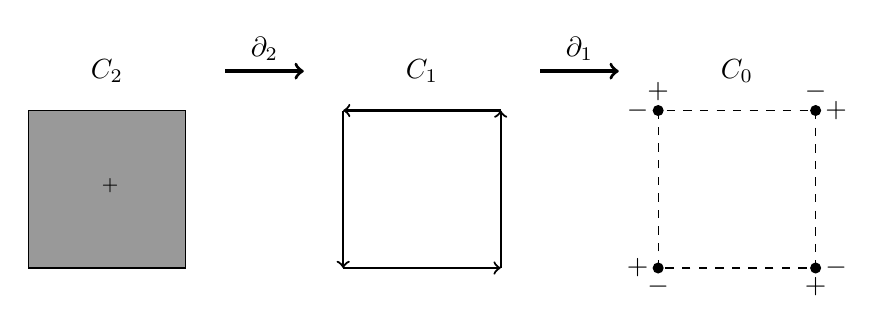
\begin{tikzpicture}
	
		\draw (1,2.5) node {$C_2$};
		\filldraw[fill=black!40] (0,0) rectangle (2,2);
		\draw (1,1) node {$\;\circlearrowleft^+$};
		
		\draw[very thick, ->] (2.5,2.5) --++ (0.5,0) node[anchor=south] {$\partial_2$} --++ (0.5,0);
		
		\draw (4+1,2.5) node {$C_1$};
		\draw[thick, ->] (4+0,0) --++ (2,0);
		\draw[thick, ->] (4+2,0) --++ (0,2);
		\draw[thick, ->] (4+2,2) --++ (-2,0);
		\draw[thick, ->] (4+0,2) --++ (0,-2);
		
		\draw[very thick, ->] (6.5,2.5) --++ (0.5,0) node[anchor=south] {$\partial_1$} --++ (0.5,0);
		
		\draw (8+1,2.5) node {$C_0$};
		\draw[dashed] (8+0,0) --++ (0,2) --++ (2,0) --++ (0,-2) --++ (-2,0);
		\fill (8,0) node[anchor=north] {$-$} node[anchor=east] {$+$} circle (2pt);
		\fill (8+2,0) node[anchor=west] {$-$} node[anchor=north] {$+$}  circle (2pt);
		\fill (8+2,2) node[anchor=south] {$-$} node[anchor=west] {$+$} circle (2pt);
		\fill (8,2) node[anchor=east] {$-$} node[anchor=south] {$+$} circle (2pt);
		
	\end{tikzpicture}
\end{figure}


Let $[\![\boldsymbol{a}, \boldsymbol{b}]\!]$ be a $k$-rectangle in $\mathbb{R}^n$.
Then we have:
\begin{align}
	\partial_k \partial_{k-1} \left( [\![ \boldsymbol{a}, \boldsymbol{b} ]\!] \right) 
	= \bigoplus_{j=1}^k (-1)^j 
		& \;  \left( \; \partial_{n-1} \left(	
			[\![ 	\boldsymbol{a}^{[\![1,n]\!]}, \;\;
				\boldsymbol{b}^{[\![1,i_j)\!)}
					\oplus \boldsymbol{a}^{[\![i_j]\!]}
					\oplus \boldsymbol{b}^{(\!(i_j,n]\!]} 
			]\!] 
		\right) \right. \notag\\[-1em]
		& \ominus \; \left. \! \partial_{n-1} \left(
			[\![ 	\boldsymbol{a}^{[\![1,i_j)\!)}
					\oplus \boldsymbol{b}^{[\![i_j]\!]}
					\oplus \boldsymbol{a}^{(\!(i_j,n]\!]} , \;\;
				\boldsymbol{b}^{[\![1,n]\!]}
			]\!] 
		\right)\right) \\[1em]
	= \bigoplus_{j=1}^k \bigoplus_{\ell=1}^{k-1} (-1)^{j+\ell}
		\;&
			[\![ 	(\boldsymbol{a}^{[\![1,n]\!]}), \;\;
				(\boldsymbol{b}^{[\![1,i_j)\!) \;\oplus\; (\!(i_j,i_{j,\ell})\!) \;\oplus\; (\!(i_{j,\ell},n]\!]}
					\oplus \boldsymbol{a}^{[\![i_j]\!] \;\oplus\; [\![i_{j,\ell}]\!]})
			]\!] \notag\\[-1em]
		\ominus \;&
			[\![ 	(\boldsymbol{a}^{[\![1,i_{j,\ell})\!) \;\oplus\; (\!(i_{j,\ell},n]\!]}
					\oplus \boldsymbol{b}^{[\![i_{j,\ell}]\!]}), \;\;
				(\boldsymbol{b}^{[\![1,i_j)\!) \;\oplus\; (\!(i_j,n]\!]}
					\oplus \boldsymbol{a}^{[\![i_j]\!]})
			]\!] \notag\\
		\ominus \; &
			[\![ 	(\boldsymbol{a}^{[\![1,i_j)\!) \;\oplus\; (\!(i_j,n]\!]}
					\oplus \boldsymbol{b}^{[\![i_j]\!]}), \;\;
				(\boldsymbol{b}^{[\![1,i_{j,\ell})\!) \;\oplus\; (\!(i_{j,\ell},n]\!]}
					\oplus \boldsymbol{a}^{[\![i_{j,\ell}]\!]})
			]\!] \notag\\
		\oplus \;&
			[\![ 	(\boldsymbol{a}^{[\![1,i_j)\!) \;\oplus\; (\!(i_j,i_{j,\ell})\!) \;\oplus\; (\!(i_{j,\ell},n]\!]}
					\oplus \boldsymbol{b}^{[\![i_j]\!] \;\oplus\; [\![i_{j,\ell}]\!]}), \;\;
				(\boldsymbol{b}^{[\![1,n]\!]})
			]\!] 
\end{align}
Note that we have $i_j$ and $i'_\ell$; after applying the first boundary operator, one dimension of the $k$-cube is degenerate.
Hence for each sequence: $\{i_j\}_{j=1}^k$ we construct $\{i_{j,\ell}\}_{\ell=1}^{k-1}$ given by:
\begin{equation}
	i_{j,1} , \ldots, i_{j,k-1} = i_1, \ldots, \widehat{i_j}, \ldots, i_k
\end{equation}
The double sum iterates over all pairs but $\oplus$ commutes so the $(k-2)$-cube with degenerate dimensions $[\![i_j]\!] \oplus [\![i_{j,\ell}]\!]$ will be iterated over twice. 
The sequences depend on one another so it is not as simple as simply swapping $\ell$ and $j$:
\begin{equation}
   [\![i_j]\!] \oplus [\![i_{j,\ell}]\!] =
     \begin{cases}
       [\![i_\ell]\!] \oplus [\![i_{\ell,j-1}]\!] & j > \ell \\
       [\![i_{\ell+1}]\!] \oplus [\![i_{\ell+1,j}]\!] & j \leq \ell
     \end{cases}
\end{equation}
So each term representing a $(k-2)$-cube will occur twice in the sum.
Once with the iteration $(j,\ell)$ and once with $(\ell, j-1)$ or $(\ell+1, j)$.
In either case, $(-1)^{j+\ell}$ is inverted meaning the two cubes will cancel.
Leaving us with the boundary of a boundary being empty.
By linearity this extends to all chains as well as the sum of empty sets is of course still empty.


\begin{definition}
	A \textbf{chain complex} is a sequence of Abelian groups $\ldots, A_2, A_1, A_0, A_{-1}, A_{-2}, \ldots$ \linebreak
	which are connected by homomorphisms $d_n:A_n \to A_{n-1}$ such that $d_n \circ d_{n+1} = 0$ for all $n$.
	Typically written out as:
	\begin{equation}
		\ldots 	\xleftarrow{d_{k-1}} A_{k-1} 
				\xleftarrow{d_{k}} A_k 
				\xleftarrow{d_{k+1}} A_{k+1} 
				\xleftarrow{d_{k+2}} \ldots
	\end{equation}
	A \textbf{cochain complex} is a sequence of Abelian groups $\ldots, A^{-2}, A^{-1}, A^0, A^{1}, A^{2}, \ldots$
	which are connected by homomorphisms $d^n:A^n \to A^{n+1}$ such that $d^n \circ d^{n-1} = 0$ for all $n$.
	Typically written out as:
	\begin{equation}
		\ldots 	\xrightarrow{d^{k-1}} A^{k-1} 
				\xrightarrow{d^{k}} A^k 
				\xrightarrow{d^{k+1}} A^{k+1} 
				\xrightarrow{d^{k+2}} \ldots
	\end{equation}
\end{definition}

$(C_\bullet, \partial_\bullet)$ is just one instance of a chain complex known as the \emph{``cubic homology''}.
In the next chapter we will look at the more general \emph{``cubic singular homology''}.
As well as the related cochain complex: the \emph{``De Rham cohomology''} and how the two relate.










%%%%%%%%%%%%%%%%%%%%%%%%%%%%%%%%%%%%%%%%%
%
% STOKE'S THEOREM
%
%%%%%%%%%%%%%%%%%%%%%%%%%%%%%%%%%%%%%%%%%
\subsection{Stokes' Theorem}

Now we come to the statement of the generalized Stokes' Theorem itself.

Given a $k-1$-form $\omega$ and $k$ chain $M$, ...

\begin{equation}
	\int_{\partial M} \omega = \int_M d\omega
\end{equation}


In one dimension this is the fundamental theorem of calculus.

In two, it is Green's Theorem and three the Kelvin-Stokes Theorem.


First we will consider Stokes theorem for the standard cube $I^k = [0,1]^k \subset \mathbb{R}^k$.
In the previous section we saw how cumbersome representing the faces in $\partial I^k$, could be.

We will denote the faces of $I^k$ by $I^k_{i=0}$ and $I^k_{i=1}$ for the $i$-th faces of $I^k$.
This allows us to rewrite:

\begin{equation}
	\partial (I^k) = \bigoplus_{i=1}^k (-1)^i \left( I^k_{i=0} \ominus I^k_{i=1} \right) 
\end{equation}

A $k-1$-form $\omega$ can be written as the sum
\begin{equation}
	\omega = \sum_{i=1}^k f_i \; dx_1 \wedge \ldots \wedge \widehat{dx_i} \wedge  \ldots \wedge dx_k
\end{equation}
but since everything: the integrals, $d$ and $\partial$ are all linear, we can work using just one of these terms.

To compute $d\omega$, we have for each term in the sum:
\begin{align*}
	d \left( f_i dx_1 \wedge \ldots \wedge \widehat{dx_i} \wedge  \ldots \wedge dx_k \right) 
 		&= df_i \wedge dx_1 \wedge \ldots \wedge \widehat{dx_i} \wedge  \ldots \wedge dx_k \\ 
 		&= \left( \sum_{j=1}^k \frac{\partial f_i}{\partial x_j} dx_j \right)
 			\wedge dx_1 \wedge \ldots \wedge \widehat{dx_i} \wedge  \ldots \wedge dx_k \\ 
\end{align*}
But for $j \neq i$, there will be a duplicate $dx_j$ term and this collision will cause the term to go to zero.
Hence only one term in the sum, $i=j$ will actually result in a non-zero term:
\begin{align*}
	d \left( f_i dx_1 \wedge \ldots \wedge \widehat{dx_i} \wedge  \ldots \wedge dx_k \right) 
 		&= \left(\frac{\partial f_i}{\partial x_i} dx_i \right)
 			\wedge dx_1 \wedge \ldots \wedge \hat{dx_i} \wedge  \ldots \wedge dx_k \\ 
		&= (-1)^{i-1} \frac{\partial f_i}{\partial x_i}
 			 dx_1 \wedge \ldots \wedge dx_k \\ 
\end{align*}
Since this is an integral over the canonical basis $\text{x} = (x_1, \ldots, x_k)$ we can remove the wedge products and
integrate as normal.
\begin{align*}
	\int_{[0,1]^k} d\omega
		=&\; (-1)^{i-1} \int_{[0,1]^k} \frac{\partial f_i}{\partial x_i}\; d(x_1, \ldots, x_k) \\
		=&\; (-1)^{i-1} \int_{[0,1]^{k-1}} \left( \int_0^1 \frac{\partial f_i}{\partial x_i} dx_i \right) 
			\;d(x_1, \ldots, \widehat{x_i}, \ldots, x_k)\\
		=&\; (-1)^{i-1}\left( \int_{[0,1]^{k-1}} f_i(x_1, \ldots, x_{i-1}, 1, x_{i+1}, \ldots, x_k)
			\;d(x_1, \ldots, \widehat{x_i}, \ldots, x_k) \right.\\
		&\;	- \left. \int_{[0,1]^{k-1}} f_i(x_1, \ldots, x_{i-1}, 0, x_{i+1}, \ldots, x_k)
			\;d(x_1, \ldots, \widehat{x_i}, \ldots, x_k) \right)
\end{align*}
The trick here being Fubini's Theorem allowing us to evaluate the iterated integral in whichever order we choose.


On the other side of the equality we have:
\begin{align*}
	\int_{\partial I^k} \omega 
		&= \sum_{j=1}^k (-1)^j \int_{I^k_{j=0}} \omega - \int_{I^k_{j=1}} \omega
\end{align*}
but $I^k_{j=0}$ is just a $k-1$ rectangle embedded in $\mathbb{R}^k$ by the map 
$(x_1, \ldots x_k-1) \mapsto (x_1, \ldots, x_{j-1}, 0, x_{j}, \ldots x_{k-1})$.
So we can think of it as just a change in coordinates.
\begin{align*}
	\int_{\partial I^k} \omega 
		&= \sum_{j=1}^k (-1)^j \int_{I^{k-1}} (I^k_{j=0})^*\omega - \int_{I^{k-1}} (I^k_{j=1})^*\omega
\end{align*}

Once we have Stokes' Theorem for the standard cube we can extend to the singular cube by:
\begin{align*}
	\int_{\partial c} \omega
		&= \int_{c (\partial ([0,1]^k))} \omega \\
		&= \int_{\partial( [0,1]^k)} c^* \omega \\
		&= \int_{[0,1]^k} dc^* \omega \\
		&= \int_{[0,1]^k} c^* d \omega \\
		&= \int_c d\omega
\end{align*}

And for a chain $C=a_1 c_1 + \ldots + a_n c_n$:
\begin{align*}
	\int_C d\omega 
		&= \int_{a_1c_1 + \ldots + a_nc_n	} d\omega \\
		&= a_1 \int_{c_1} d\omega + \ldots + a_n \int_{c_n} d\omega \\
		&= a_1 \int_{\partial c_1} \omega + \ldots + a_n \int_{\partial c_n} \omega \\
		&= \int_{a_1 \partial c_1 + \ldots a_n \partial c_n} \omega \\
		&= \int{\partial ( a_1c_1 + \ldots + a_n c_n)} \omega \\
		&= \int_{\partial C} \omega
\end{align*}


\section{Applications}

\subsection{Integrating a mesh}

\begin{equation}
	f(x,y) = \frac{\sin(x) \cos(y)}{\cos^2(x) + \sin^2(x)}
\end{equation}

Anti-periodic $f(x+P) = -f(x)$

\subsection{Irrational numbers}

\subsection{Contour Integral}







